%external contents box

\newtcolorbox{externalcontent}[1][]{
    enhanced,
    sidebyside,
    lefthand width=1.5cm,
    bicolor,
    colback=black!10,
    colbacklower=black!2,
    notitle,
    sharp corners,
    boxrule=1pt,
    borderline west={2mm}{0mm}{black},
    width=.9\linewidth,
    center,
    #1
    }    

\newenvironment{pythonexc}
    {
    \begin{externalcontent}[width=.9\linewidth]
    
\includegraphics[width=\textwidth]{Images/icon_python.pdf}
    \tcblower
    }
    {
    \end{externalcontent}
    }

\newenvironment{datasetexc}
    {\begin{externalcontent}[width=.9\linewidth]
    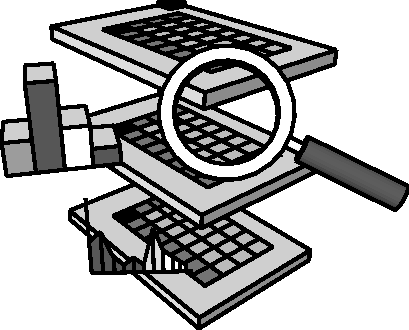
\includegraphics[width=\textwidth]{Images/icon_dataset2.pdf}
    \tcblower
    }
    {
    \end{externalcontent}
    }

\newenvironment{jupyterexc}
    {\begin{externalcontent}[width=.9\linewidth]
    
\includegraphics[width=\textwidth]{Images/icon_jupyter.pdf}
    \tcblower
    }{
    \end{externalcontent}
    }
    
\newenvironment{freecadexc}
    {\begin{externalcontent}[width=.9\linewidth]
    
\includegraphics[width=\textwidth]{Images/icon_freecad.pdf}
    \tcblower
    }{
    \end{externalcontent}
    }